\documentclass[12pt,a4paper]{article}

% Language setting
\usepackage[portuguese]{babel}
%\addto\captionsportuguese{\newcommand{\andname}{e}}

% Set page size and margins
\usepackage[a4paper,top=2cm,bottom=2cm,left=2.5cm,right=2.5cm,marginparwidth=1.75cm]{geometry}


\usepackage{amsmath}
\usepackage{graphicx}
\usepackage[colorlinks=true, allcolors=blue]{hyperref}
\usepackage{hyperref}
\usepackage{orcidlink}
\usepackage[title]{appendix}
\usepackage{mathrsfs}
\usepackage{amsfonts}
\usepackage{booktabs} % For \toprule, \midrule, \botrule
\usepackage{caption}  % For \caption
\usepackage{threeparttable} % For table footnotes
\usepackage{listings}
\usepackage{enumitem}
\usepackage{chngcntr}
\usepackage{booktabs}
\usepackage{lipsum}
\usepackage{subcaption}
\usepackage{authblk}
\usepackage[T1]{fontenc}    % Font encoding
\usepackage{csquotes}       % Include csquotes
\usepackage{diagbox}


% Customize line spacing
\usepackage{setspace}
\onehalfspacing % 1.5 line spacing

% Redefine section and subsection numbering format
\usepackage{titlesec}
\titleformat{\section} % Redefine section numbering format
  {\normalfont\Large\bfseries}{\thesection.}{1em}{}

% Change the position of the table caption above the table
\usepackage{float}   % for customizing caption position
\usepackage{caption} % for customizing caption format
\captionsetup[table]{position=top} % caption position for tables

% Define the unnumbered list
\makeatletter
\newenvironment{unlist}{%
  \begin{list}{}{%
    \setlength{\labelwidth}{0pt}%
    \setlength{\labelsep}{0pt}%
    \setlength{\leftmargin}{2em}%
    \setlength{\itemindent}{-2em}%
    \setlength{\topsep}{\medskipamount}%
    \setlength{\itemsep}{3pt}%
  }%
}{%
  \end{list}%
}
\makeatother

% Suppress the warning about \@parboxrestore
\pdfsuppresswarningpagegroup=1

%-------------------------------------------
% Paper Head
%-------------------------------------------
\title{PTC3314 - Ondas e Linhas}
\author{4º Exercício de Simulação Computacional}

\affil{Guilherme Fortunato Miranda, Nº USP: 13683786}
\affil{João Pedro Dionizio Calazans, Nº USP: 13673086}
\affil{Thomas de Castro Hess, Nº USP: 11806090}
\affil{Turma 02 – Grupo B}

\date{08 de Dezembro de 2024}

\begin{document}

\maketitle

\paragraph{a)}

$\theta_c=30,92641^\circ$

\begin{center}
    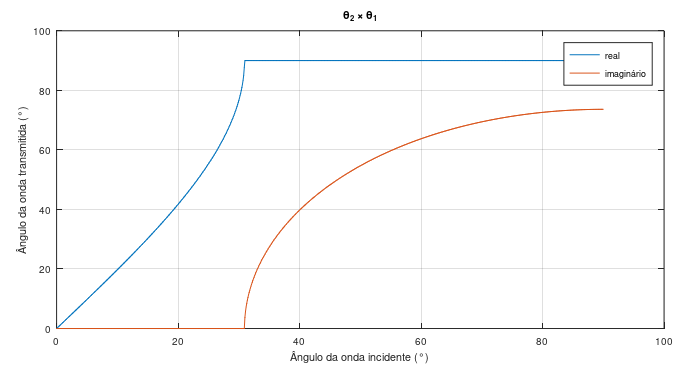
\includegraphics[scale=.9]{item a.png}
\end{center}

\paragraph{b)}

$Z_L(0^\circ)=376,73\ \Omega$

$\ \ Z_L(\theta_c)=0,0\ \Omega$

$\ \ Z_L(90^\circ)=-j628,82\ \Omega$

\begin{center}
    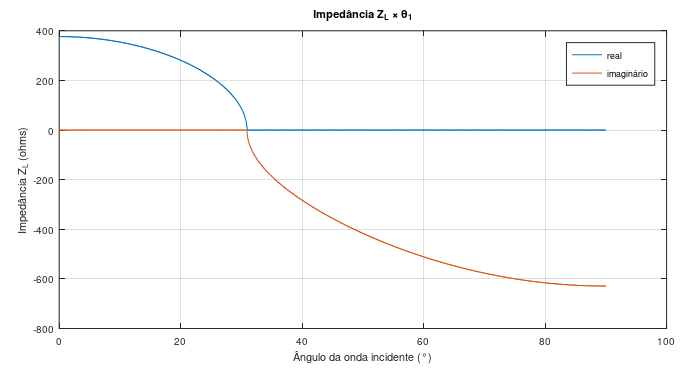
\includegraphics[scale=.9]{item b.png}
\end{center}

\paragraph{c)}

$\theta_p=27,2^\circ$

% \hspace{-1.5cm}
    \begin{tabular}{llll}
         Potência transmitida: &$\left.\frac{|N^+_{z2}|}{|N^+_{z1}|}\right|_{\theta_i=0^\circ}=0,89692$&$ \left.\frac{|N^+_{z2}|}{|N^+_{z1}|}\right|_{\theta_i=\theta_p}=1$&$\left.\frac{|N^+_{z2}|}{|N^+_{z1}|}\right|_{\theta_i=\theta_c}=0$\\

         
         Potência refletida: &$\left.\frac{|N^-_{z1}|}{|N^+_{z1}|}\right|_{\theta_i=0^\circ}=0,10308$&$ \left.\frac{|N^-_{z1}|}{|N^+_{z1}|}\right|_{\theta_i=\theta_p}=0$&$\left.\frac{|N^-_{z1}|}{|N^+_{z1}|}\right|_{\theta_i=40^\circ}=1$\\
    \end{tabular}

\begin{center}
    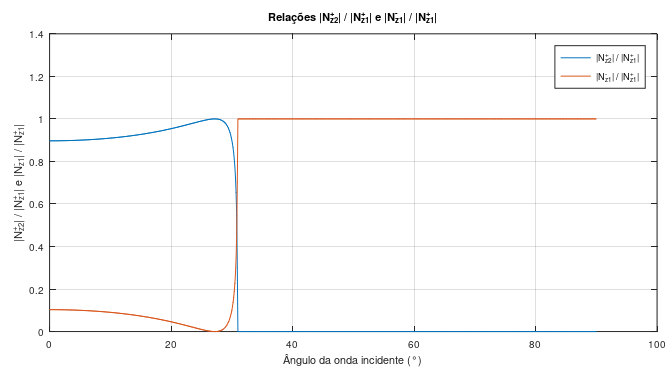
\includegraphics[scale=.9]{item c.png}
\end{center}

\break

\paragraph{d)}

$|\dot H_y(z=0)|=0,37231\ mA_{ef}/m$

$\ \ |\dot H_y(z=5cm)|=0,089878\ mA_{ef}/m$

\begin{center}
    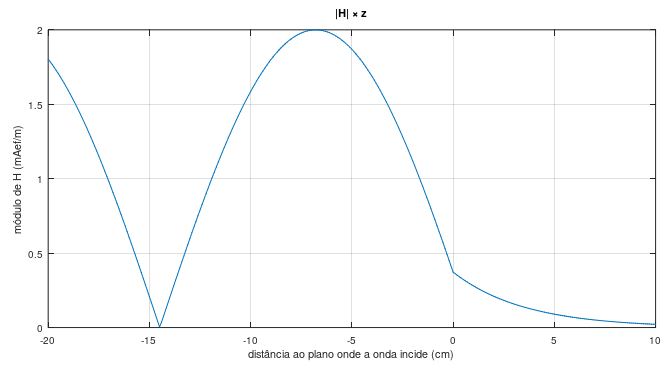
\includegraphics[scale=.9]{item d.png}
\end{center}

\vspace{1.5cm}
\hspace{-2.5cm}

\includegraphics[scale=.6]{happy.png}

\end{document}